\documentclass[11pt,spanish,a4paper]{article}
% Versión 1.er cuat 2021 Víctor Bettachini < bettachini@df.uba.ar >

% Versión 1.er cuat 2021 Víctor Bettachini < bettachini@df.uba.ar >

\usepackage[T1]{fontenc}
\usepackage[utf8]{inputenc}

\usepackage[spanish, es-tabla]{babel}
\def\spanishoptions{argentina} % Was macht dass?
% \usepackage{babelbib}
% \selectbiblanguage{spanish}
% \addto\shorthandsspanish{\spanishdeactivate{~<>}}

\usepackage{graphicx}
\graphicspath{{./figuras/}}
% \usepackage{float}

\usepackage[arrowdel]{physics}
\newcommand{\pvec}[1]{\vec{#1}\mkern2mu\vphantom{#1}}
% \usepackage{units}
\usepackage[separate-uncertainty=true, multi-part-units=single, locale=FR]{siunitx}
\usepackage{isotope} % $\isotope[A][Z]{X}\to\isotope[A-4][Z-2]{Y}+\isotope[4][2]{\alpha}

\usepackage{tasks}
\usepackage[inline]{enumitem}
% \usepackage{enumerate}

\usepackage{hyperref}

% \usepackage{amsmath}
% \usepackage{amstext}
\usepackage{amssymb}

\usepackage{tikz}
\usepackage{tikz-dimline}
\usetikzlibrary{math}
\usetikzlibrary{arrows.meta}
% \usetikzlibrary{snakes}
% \usetikzlibrary{calc}
\usetikzlibrary{decorations.pathmorphing}
\usetikzlibrary{patterns}

\usepackage[hmargin=1cm,vmargin=1.6cm,nohead]{geometry}
% \voffset-3.5cm
% \hoffset-3cm
% \setlength{\textwidth}{17.5cm}
% \setlength{\textheight}{27cm}

\usepackage{lastpage}
\usepackage{fancyhdr}
\pagestyle{fancyplain}
\fancyhead{}
\fancyfoot{{\tiny \textcopyright DF, FCEyN, UBA}}
\fancyfoot[C]{ {\tiny Actualizado al \today} }
\fancyfoot[RO, LE]{Pág. \thepage/\pageref{LastPage}}
\renewcommand{\headrulewidth}{0pt}
\renewcommand{\footrulewidth}{0pt}


\begin{document}
\begin{center}
\textbf{Física 2} (Físicos) \hfill \textcopyright {\tt DF, FCEyN, UBA}\\
	\textsc{\LARGE Sistemas con dos grados de libertad}
\end{center}


Los ejercicios con (*) entrañan una dificultad adicional y puede considerarlos opcionales.

\begin{enumerate}


\item
\begin{minipage}[t][5cm]{0.75\textwidth}
\textbf{Resortes colgantes}.
Asuma que el sistema de la figura no está bajo el efecto de un campo gravitatorio
\begin{enumerate}
	\item Obtenga sus frecuencias naturales de oscilación y los modos normales correspondientes.
	Escriba las ecuaciones de movimiento de cada partícula.
	\item Sabiendo que a $t= 0$ el sistema satisface las siguientes condiciones: $\Psi_a(0)= 1, \, \Psi_b(0)= 0$ y que se encuentra en reposo, encuentre el movimiento de cada partícula.
	\item Analice cómo se modifica el resultado por la presencia de la gravedad en la superficie de la Tierra.
\end{enumerate}
\end{minipage}
\begin{minipage}[c][0cm][t]{0.2\textwidth}
  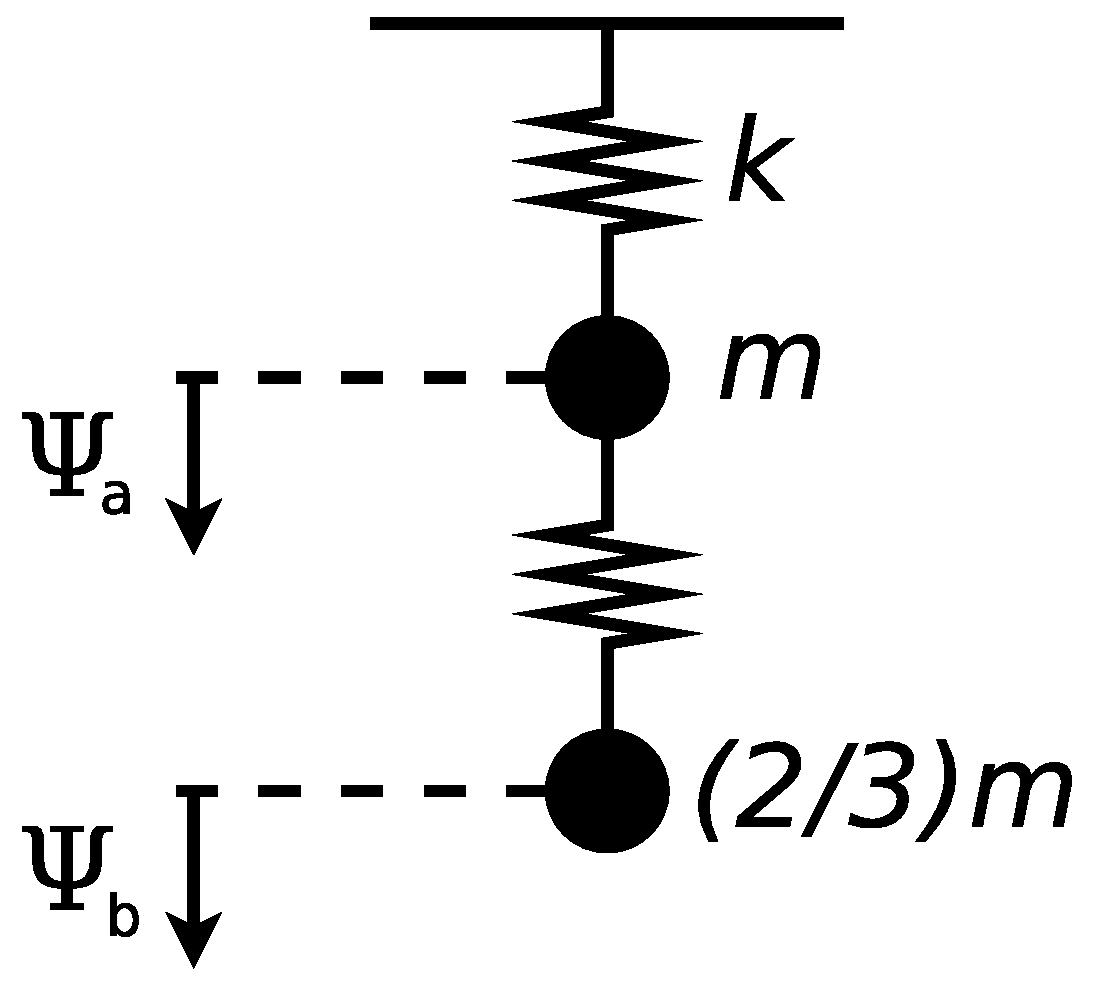
\includegraphics[width=\textwidth]{ej1-6}
\end{minipage}



\item
\begin{minipage}[t][3cm]{0.6\textwidth}
En el sistema de la figura se tienen dos partículas de masa $m$ unidas a las paredes con resortes dispuestos verticalmente de longitud natural $l_0$ ($l_0< L/2$) y constante elástica $k_1$, y con otros dispuestos horizontontalmente de $l_0= 0$ (\emph{slinkies}) y constante $k_2$.
Imagine que las partículas tienen la libertad de moverse en el plano y que el sistema no está en un campo gravitatorio.
\end{minipage}
\begin{minipage}[c][1cm][t]{0.35\textwidth}
  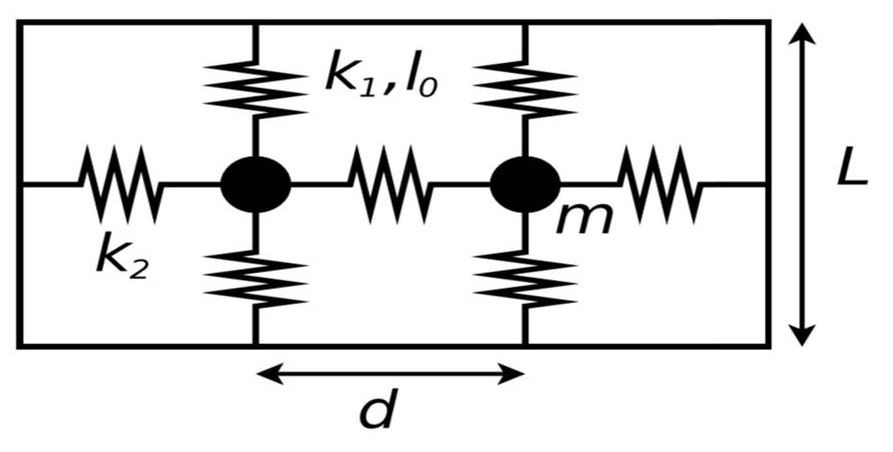
\includegraphics[width=\textwidth]{resortes_acoplados}
\end{minipage}
\begin{enumerate}
	\item ¿Bajo qué aproximaciones es posible decir que el movimiento más general posible de cada una de las masas es una superposición lineal del movimiento más general posible de las oscilaciones longitudinales y de las oscilaciones transversales?
	Demuestre su afirmación.
	\item Considerando la aproximación del punto anterior, determine las frecuencias propias y los modos normales de oscilación: longitudinales, transversales y de la solución más general posible para un movimiento arbitrario en el plano.
\end{enumerate}



\item \label{pendacop}
\begin{minipage}[t][4cm]{0.75\textwidth}
De dos péndulos de igual longitud $l$ penden pesos de masas diferente $m_a$ y $m_b$.
Estas están acopladas entre sí mediante un resorte de constante elástica $k$.
\begin{enumerate}
	\item Escriba las ecuaciones de movimiento de cada masa. considerando pequeñas oscilaciones, ¿es relevante considerar $l_0 \neq 0$?
	¿Qué cambia si el resorte es \emph{slinky}?   
	\item Obtenga las frecuencias naturales del sistema y sus modos normales de oscilación.
	Interprete el significado físico de estos modos normales. 
\end{enumerate}
\end{minipage}
\begin{minipage}[c][0cm][t]{0.2\textwidth}
  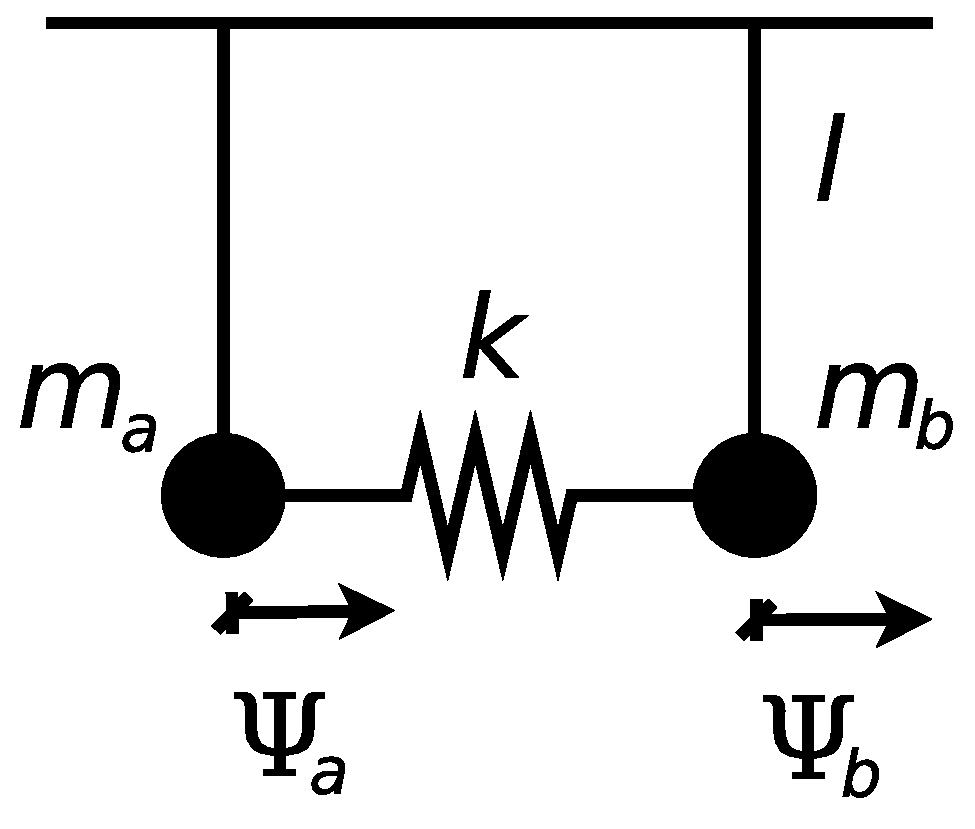
\includegraphics[width=\textwidth]{ej1-7}
\end{minipage}



\item \label{2masitas}
\begin{minipage}[t][2cm]{0.65\textwidth}
Dos pesas de idéntica masa están apoyadas en una mesa sin rozamiento, sujetas a las paredes por resortes de constante
elástica $k$ y unidas entre sí por otro con distianta constante $k'$.
Obtenga las frecuencias y los modos transversales del sistema. 
\end{minipage}
\begin{minipage}[c][0.5cm][t]{0.3\textwidth}
  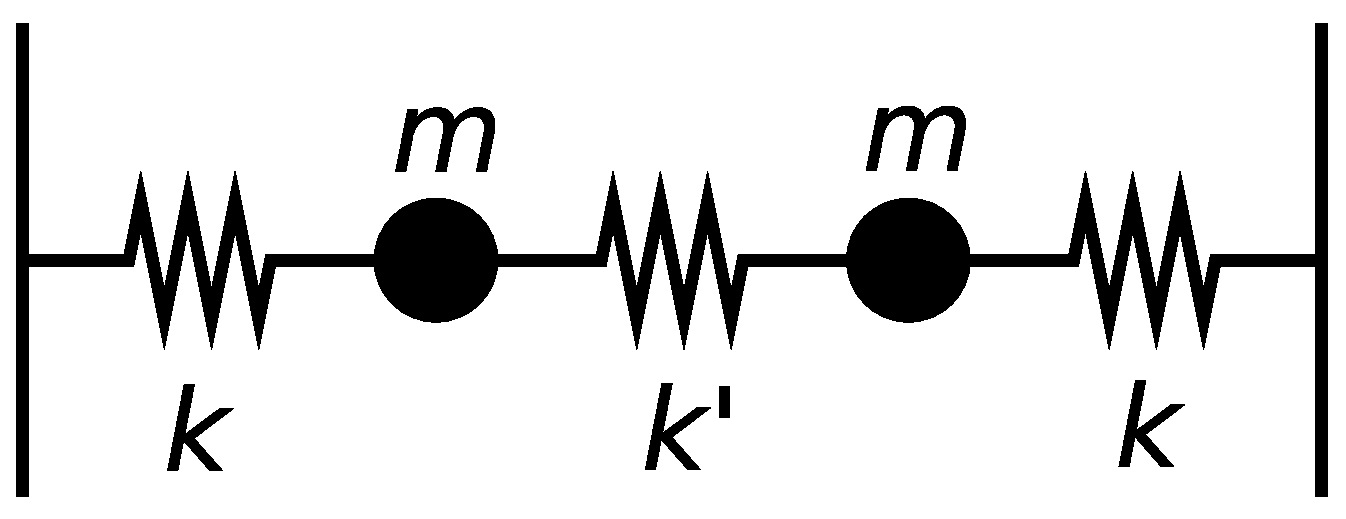
\includegraphics[width=\textwidth]{ej1-8}
\end{minipage}



\end{enumerate}

\end{document}
